\documentclass[pdf,aspectratio=169]{beamer}
\usepackage[]{hyperref,graphicx,siunitx,lmodern,booktabs,tikz,tensor}
\usepackage{pdfpc-commands}
\usepackage{pgfplots, pgfplotstable}
\usepackage[mode=buildnew]{standalone}
\mode<presentation>{\usetheme{Astro}}

\graphicspath{ {../Images/} }

\sisetup{per-mode=symbol}
\usetikzlibrary{calc,intersections, decorations.pathmorphing,shadings}
%\tikzstyle{proton}=[circle, minimum size = 7mm, ball color=red, black,transform shape]
%\tikzstyle{neutron}=[circle, minimum size=7mm, ball color=gray, black, transform shape]
%\tikzstyle{gammaray}=[ultra thick, -latex, decorate, decoration={snake, post length=3mm}]


%preamble
\title{Gimme an H! Gimme an R!}
\date{October 31, 2018}
\author{Jed Rembold}

\begin{document}
\renewcommand*{\theenumi}{\Alph{enumi}}

\begin{frame}{Announcements}
	\begin{itemize}
		\item Webwork due on Friday
		\item I'm looking to get new grade reports issued
		\item I'll hand Test 2 back on Friday
		\item Test 3 will be 2 weeks from Friday (the Friday before Thanksgiving)
		\item Polling: \url{rembold-class.ddns.net}
	\end{itemize}
\end{frame}

\begin{frame}{End of an Era}
	\begin{itemize}
		\item The Kepler Space Telescope has run out of fuel
			\begin{itemize}
				\item Can no longer reorient itself to point at certain objects
			\end{itemize}
		\item Orbits the Sun, not Earth
		\item History
			\begin{itemize}
				\item Launched in 2009
				\item Originally stared at a single patch of sky
				\item In 2013 a reaction wheel failed, but was able to compensate using sunlight pressure
				\item Switched to K2 mode just looking at interesting things
			\end{itemize}
		\item Found 2,327 confirmed exoplanets with about 2,900 still to confirm
		\item Work is taken over largely by TESS, the Transiting Exoplanet Survey Satellite
	\end{itemize}
\end{frame}

\begin{frame}{Understanding Check!}
  Jupiter is 12 times brighter than Vega while Venus is approximately 60 times brighter than Vega. What is the difference between the apparent magnitudes of Jupiter and Venus ($m_V - m_J$)
  \begin{enumerate}
	\item \alert<2>{-1.7}
	\item -0.7
	\item 0.2
	\item 5
  \end{enumerate}
\end{frame}

%\begin{frame}{Luminosity}
  %\begin{columns}
	%\column{.5\textwidth}
	%\begin{itemize}
	  %\item We measure the apparent brightness $B$
	  %\item Brightness falls off with distance:
		%\[B = \frac{L}{4\pi d^2}\]
	  %\item Thus the luminosity is
		%\[L = 4\pi d^2 \times B\]
	  %\item Range of stellar luminosities is large:
		%\begin{itemize}
		  %\item $L_{Sun}$ = \SI{4e26}{\watt}
		  %\item Dimmest at $0.000001 L_{Sun}$
		  %\item Brightest at $100000 L_{Sun}$
		%\end{itemize}
	%\end{itemize}
	%\column{.5\textwidth}
	%\begin{center}
	  %\begin{tikzpicture}
		%\clip (0,0) circle (2.54cm);
		%\node at (0,0) {\includegraphics[width=\textwidth]{ch12_LightFalloff.png}};
	  %\end{tikzpicture}
	%\end{center}
  %\end{columns}
%\end{frame}

\begin{frame}{Refresher}
  We wanted to be able to find:
	\begin{itemize}
	  \item \alert<2->{Surface Temperature}
	  \item \alert<2->{Motion}
	  \item Distance (sometimes)
	  \item Size (in a way)
	  \item \alert<3->{Power output (Luminosity)}
	  \item Mass (also sometimes)
	\end{itemize}
\end{frame}

\begin{frame}{Star Sizes}
  \begin{itemize}
	\item We've mentioned that we can \emph{not} resolve most stars
	\item We can get the size in a sneaky way though!
	  \begin{itemize}
		\item Stefan-Boltzmann law and Luminosity:
		  \begin{align*}
			L &= 4\pi R^2 \times I \\
			&= 4\pi R^2 \times \sigma T^4
		  \end{align*}
	  \end{itemize}
	\item A \textcolor{red!70!black}{cooler} star can have a high luminosity if it is {\LARGE large}
	\item A \textcolor{blue!40}{hot} star can have a low luminosity if it is {\scriptsize small}
  \end{itemize}
\end{frame}


\begin{frame}{Stellar Distances}
  \begin{itemize}
	\item Back to parallax!
	\item Still the only real method we have to determine distances to stars
	\item Recall parallax effects are larger for closer objects
	  \begin{itemize}
		\item We need as large a baseline as we can get: observe during 6 month intervals
		\item The parallax effects from stars are still tiny!
		\item Generally less than an arcsecond
	  \end{itemize}
	\item A \alert{Parsec} is the distance that corresponds to a parallax angle of 1 arcsecond
	  \begin{itemize}
		\item Equivalent to 3.26 light years
	  \end{itemize}
	\item Measuring the parallax angle ($p$) in arcseconds yields
	  \[d = \frac{1}{p}\]
	  where $d$ is in parsecs. 
  \end{itemize}
\end{frame}

\begin{frame}{Driving to Vega(s)}
  \begin{example}
	You measure the parallax angle of the star Vega to be \ang{;;0.13014}. If you were to drive at the speed of light, how long would it take you to get to Vega?
  \end{example}
\end{frame}

\begin{frame}{Stellar Masses}
  \begin{itemize}
	\item Almost all information on mass comes from Kepler's 3rd law
	\item Need another massive object to be rotating around $\Rightarrow$ Binary Systems
  \end{itemize}
  \begin{center}
	\includegraphics[width=.7\textwidth]{ch12_binary-star-system.jpg}
  \end{center}
\end{frame}

\begin{frame}{Binaries and Kepler}
  \begin{itemize}
	\item Recall that binary stars orbit about the center of mass
	\item Both stars have the same period
	\item By fancy application of Kepler's 3rd:
	  \[\frac{a_{AU}^3}{P_{yr}^2} = (M_1 + M_2)_{\odot}\]
	  \begin{itemize}
		\item $a$ is the average separation of the stars in AU
		\item $P$ is the orbital period in years
		\item $\odot$ indicates the masses are in ``Solar Mass'' units. (eg. $5M_{\odot}$ is 5 times the mass of the Sun)
	  \end{itemize}
	\item Careful observations of both stars can result in finding the center of mass point, and thus finding the mass of both stars
  \end{itemize}
\end{frame}

\begin{frame}{Round and Round}
  \begin{example}
	What is the combined mass of the below binary system? Each grid line is 1 AU.
	\begin{center}
	  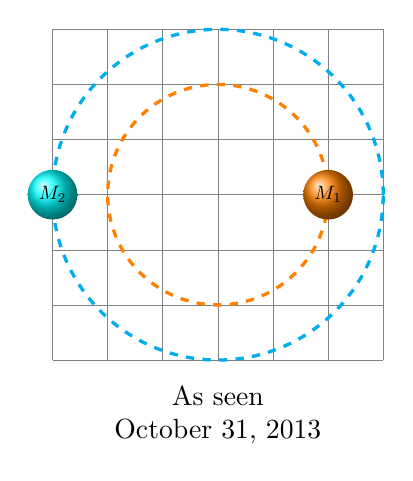
\begin{tikzpicture}[scale=.7]
		\draw[help lines] (-3,-3) grid (3,3);
		\draw[orange, dashed, very thick] (0,0) circle (2cm);
		\node[circle, ball color=orange, text=black, transform shape] at (0:2) {$M_1$};
		\draw[cyan, dashed, very thick] (0,0) circle (3cm);
		\node[circle, ball color=cyan, text=black, transform shape] at (180:3) {$M_2$};
		\node[align=center] at (0,-4) {As seen\\October 31, 2013};
	  \end{tikzpicture}
	  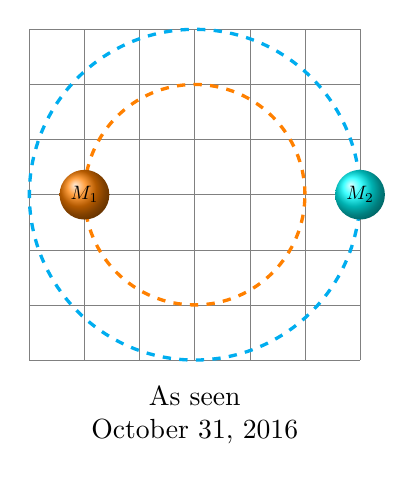
\begin{tikzpicture}[scale=.7]
		\draw[help lines] (-3,-3) grid (3,3);
		\draw[orange, dashed, very thick] (0,0) circle (2cm);
		\node[circle, ball color=orange, text=black, transform shape] at (180:2) {$M_1$};
		\draw[cyan, dashed, very thick] (0,0) circle (3cm);
		\node[circle, ball color=cyan, text=black, transform shape] at (0:3) {$M_2$};
		\node[align=center] at (0,-4) {As seen\\October 31, 2016};
	  \end{tikzpicture}
	\end{center}
  \end{example}
\end{frame}

\begin{frame}{Example: Sirius A and B}
  \begin{itemize}
	\item An interesting visual binary system:
	  \begin{itemize}
		\item A is 10000 times brighter than B
		\item B is twice as hot
	  \end{itemize}
	  \begin{center}
		\includegraphics[width=5cm]{ch12_Sirius1.jpg}
		\includegraphics[width=4.75cm]{ch12_Sirius2.jpg}
	  \end{center}
	\item We observe: spectra, parallax, angular separation, period
	\item We can infer: temperature, distance, physical separatiaon, mass, luminosity, and SIZE
  \end{itemize}
\end{frame}

\begin{frame}{Sirius\ldots Black?}
  \begin{itemize}
	\item Found that Sirius B is \alert{really} small
	  \begin{itemize}
		\item Smaller than the Earth
		\item As massive as the Sun
	  \end{itemize}
	\item Really confused early astronomers!
	\item Arthur Eddington:
	  \begin{quote}
		The message of the Companion of Sirius when it was decoded ran: \alert{``I am composed of material 3,000 times denser than anything you have come across; a ton of my material would be a little nugget that you would put in a matchbox.''}
		What reply can one make to such a message? The reply that most of us made in 1914 was: \alert{``Shut up. Don't talk nonsense.''}
	  \end{quote}
  \end{itemize}
\end{frame}

%\begin{frame}{Understanding Check}
  %What is the combined mass of the below system? Each grid is 1 AU.
  %\begin{center}
	%\begin{tikzpicture}
	  %\draw[help lines] (-3,2) grid (6,-2);
	  %\draw[orange] (0,0) ellipse (3cm and 2cm);
	  %\draw[cyan] (3,0) ellipse (3cm and 2cm);
	  %\node[circle, ball color=orange, text=black] at (-3,0) {\tiny 2012};
	  %\node[circle, ball color=cyan, text=black] at (6,0) {\tiny 2012};
	  %\node[circle, ball color=orange, text=black] at (3,0) {\tiny 2016};
	  %\node[circle, ball color=cyan, text=black] at (0,0) {\tiny 2016};

	  %\node at (-3,-3) {A. $0.4M_\odot$};
	  %\node at (0,-3) {\alert<2>{B. $3.4M_\odot$}};
	  %\node at (3,-3) {C. $11.4M_\odot$};
	  %\node at (6,-3) {D. $13.5M_\odot$};
	%\end{tikzpicture}
  %\end{center}
%\end{frame}


\begin{frame}{Hertzsprung-Russel Diagrams}
  \begin{center}
	\begin{tikzpicture}
	  \pgfplotsset{colormap={stars}{[0.1cm] color(0cm)=(blue); color(1.8cm)=(white); color(2.1cm)=(yellow); color(2.6cm)=(red); color(3cm)=(red!50!black)}}
	  \begin{loglogaxis}[
		  width=\textwidth,
		  height=7.5cm,
		  x dir = reverse,
		  xlabel = Temperature (K),
		  ylabel = Fraction of Sun's Luminosity,
		  ticklabel style={font=\tiny},
		  xtick = {3000, 6000, 10000, 25000},
		  xticklabels = {3000,6000,10000,25000},
		  colormap name= stars,
		]
		\addplot[scatter, scatter src=-x, draw=black, only marks, mark size = 1pt] table[x index=0, y index=1] {../Data/HR_Data.csv};
		\node at (axis cs: 10^4.5,10^-4) {O};
		\node at (axis cs: 10^4.2,10^-4) {B};
		\node at (axis cs: 10^3.95,10^-4) {A};
		\node at (axis cs: 10^3.85,10^-4) {F};
		\node at (axis cs: 10^3.7,10^-4) {G};
		\node at (axis cs: 10^3.6,10^-4) {K};
		\node at (axis cs: 10^3.4,10^-4) {M};
	  \end{loglogaxis}
	  %\draw[orange] (0,0) grid (9,6);
	  \path<2> (2,4) -- node[midway,sloped, rounded corners, fill=white, fill opacity = 0.7, text=black, text opacity =1] {Main Sequence} (7,1.5);
	  \node<3>[rounded corners, fill=white, fill opacity=0.7, text=black, text opacity=1] at (2.5,1) {White Dwarfs};
	  \node<4>[rounded corners, fill=white, fill opacity=0.7, text=black, text opacity=1] at (7,3.5) {Giants};
	  \node<5>[rounded corners, fill=white, fill opacity=0.7, text=black, text opacity=1] at (6,5) {Supergiants};
	\end{tikzpicture}
  \end{center}
\end{frame}

\begin{frame}{Patterns in HR Diagrams}
  \begin{itemize}
	\item Hot, Bright stars in upper left
	\item Cool, dim stars in lower right
	\item Luminosity depends on both temperature and size
	  \begin{itemize}
		\item Size increases toward the upper right
	  \end{itemize}
	\item Most stars lie along the Main Sequence
	\item How does mass come into it?
  \end{itemize}
\end{frame}

\begin{frame}{Mass and HR Diagrams}
  \begin{itemize}
	\item Globally, there is not an obvious trend
	\item Trends are clear though for subgroups:
	  \begin{itemize}
		\item Main sequences stars decrease in mass from upper left to lower right
		\item White dwarfs are all generally low mass
		\item Giants and Supergiants can be any mass
	  \end{itemize}
	\item Mass determines where the balance point between energy in and energy out lies
	  \begin{itemize}
		\item More mass implies hotter and denser fusion and thus more energy
		\item Also influences how large the star is
		\item Lots of interacting systems striving for balance
	  \end{itemize}
  \end{itemize}
\end{frame}

\begin{frame}{Not much for Vacations}
  \begin{columns}
	\column{.5\textwidth}
	\begin{itemize}
	  \item Stars tend to live most their lives in one place on the main sequence
	  \item Stars do not (significantly) change mass over their lifetimes
	\end{itemize}
	\column{.5\textwidth}
	\begin{center}
	  \begin{tikzpicture}
		\clip[rounded corners] (1mm,3mm) rectangle +(68mm,68mm);
		\node[inner sep=0pt, outer sep=0pt, anchor=south west] at (0,0) {\includegraphics[width=7cm]{ch12_lifetimes.jpg}};
	  \end{tikzpicture}
	\end{center}
  \end{columns}
\end{frame}

\begin{frame}{Shine Bright \scriptsize(like a diamond)}
  \begin{columns}
	\column{.5\textwidth}
	\begin{center}
	  \begin{tikzpicture}
		\clip[rounded corners] (1mm,3mm) rectangle +(68mm,68mm);
		\node[inner sep=0pt, outer sep=0pt, anchor=south west] at (0,0) {\includegraphics[width=7cm]{ch12_lifetimes.jpg}};
	  \end{tikzpicture}
	\end{center}
	\column{.5\textwidth}
	\begin{itemize}
	  \item A star's mass and luminosity do not increase at the same rate:
		\begin{itemize}
		  \item O star
			\begin{itemize}
			  \item $60 M_\odot$
			  \item $100000 L_\odot$
			\end{itemize}
		  \item G star
			\begin{itemize}
			  \item $1 M_\odot$
			  \item $1 L_\odot$
			\end{itemize}
		  \item M star
			\begin{itemize}
			  \item $0.2 M_\odot$
			  \item $0.01 L_\odot$
			\end{itemize}
		\end{itemize}
	  \item Brighter stars have shorter lifetimes than dimmer stars!
	\end{itemize}
  \end{columns}
\end{frame}

%\begin{frame}{The End of the Line}
  %\begin{itemize}
	%\item What about those stars not on the main sequence?
	%\item Fusing hydrogen into helium does not account for them
	%\item $\Rightarrow$Stars that have exhausted their supply of hydrogen
	%\item Two main types:
	  %\begin{itemize}
		%\item Giants
		  %\begin{itemize}
			%\item In crisis mode: ``Fuse all the things!''
		  %\end{itemize}
		%\item Dwarfs
		  %\begin{itemize}
			%\item In dejection, having lost all their fuel
			%\item Memories of once being a Giant
		  %\end{itemize}
	  %\end{itemize}
  %\end{itemize}
%\end{frame}






\end{document}
